\documentclass[12px]{article}
% \usepackage{amsmath}
\usepackage[fleqn]{amsmath}
\usepackage{amssymb}
\usepackage{graphicx}
\usepackage{cancel}
\usepackage{biblatex}

\addbibresource{bib_file.bib}
\graphicspath{ {./images/} }

\newcommand{\R}{\mathbb{R}}


\begin{document}

    \title{ECH 267 Nonlinear Control Theory \\ Project Abstract }

    \author{Jonathan Dorsey: Department of Mechanical \& Aerospace Engineering}

    \maketitle


    \section*{Project Overview}

    The objective of this project is to implement an optimal \underline{Path Planner} using Model Predictive Control (MPC). The target system used in this project will be a robotic arm. The responsibility of the MPC controller/planner will be to generate the `optimal' path, from a specified starting waypoint to a specified ending waypoint, as well as facilitate the control of the arm from the current position to the next. This formulation should be able to use MPC as a near-online means of generating optimal paths, in real-time, as well as avoid obstacles, which might exist in the robots workspace.

    \section*{Background \& Motivation:}

    Since my undergraduate studies, robotics has been a field that I want to keep exploring both personally and professionally. The interesection of control systems, software \& algorithms, with the domains of mechanical and electrical system in such a way as to manipulate physical system to perform desired functions has always intrigued me. Secondly, even though I have taken an optimal controls course, (due to CA fires \& class cancellation) I have never implemented Model Predictive Control from scratch before, without using tools that dissasociate the concept of MPC with the implementation of MPC such as the \underline{MatLab MPC Toolbox}. Since I do not believe that my currently research is terribly compatible with nonlinear systems/control (Lyapunov or Optimal), I envision this course project as the medium through which I can explore my interest in robotics with my desire to understand and implement nontrivial control methodologies, on complex systems, to a level of depth which I have not been able to obtain in previous studies.

    \pagebreak

    \section*{Topic \& Course Relevance:}


    The overarching topic of this project is \underline{Path Planning and control using MPC}, on a robotic manipulator. Unlike trajectory generation, path planning does not present the concept of track a position in space with resect to time. Therefore \underline{path planning} is a more obtainable goal to reach for. However, by the vary nature of the MPC formulation, we can penalize the time that it takes the robot to transition from one position to the next, effectively forming a time metric for the path planner and control. Since MPC is a predictive algorithm, the optimized path/trajectory can only see as far ahead in time as the prediction horizon. This means that the path is generated piecewise in time, and that the \textbf{optimal path} might necessitate recalculation multiple times. This is espcially true if there are disturbances, model-plant mismatch, or other factors which cause the controller to keep correcting the system according to feedback. \\

    \noindent However, the main elements of this project can be categorized into one of the following sub-topics, which perfectly align with the course objectives of ECH-267.

    \begin{enumerate}
        \item Nonlinear Dynamic System (Robot Arm)
        \item Model Predictive Control (for Planning \& Control)
    \end{enumerate}

    \noindent Each of these sub-topics have fair extensive literature written about them. However, in my research for this project, I found that while each component was very well studied, the coupling of optimal path planning (via MPC) and robotic manipulators was fairly limited. \cite{chao} Much of the existing research in this field is either not based on the MPC formulation and relies on other optimization based methods, or other approaches such as artificial potential fields, or that the trajectory/path prediction and planning problems are typically cast into a discretized formulation where graph search algorithms such as $A^*$, Dijkstra's algorithm, probabilistic road maps, rapidly-exploring-random-trees(RRT/$RRT^*$), and other discrete space/graph/heuristic search techniques, are more commonly applied. \\

    \noindent However, the coupling of these two topics is perfectly matched for the ciriculum of this course. It pairs a highly nonlinear physical system with the desire to plan and control the behavior of that system. In fact, using the optimal path given by the MPC controller, it is also possible to compare hybrid control methodologies (obtain path via MPC but track the reference via some other controller paradigm) and the benefit they have on controlling nonlinear systems. A comparison of nonlinear controllers given the optimal trajectory/path could include MPC against sliding mode control, PID, LQR...etc.


    \pagebreak


    \section*{Project Objectives}

    It is important to define the objectives and goals for the project as these provide the scope of the problem being solved, highlights primary issues to address, and provide a metric for completion. With this in mind the following objectives are an attempt to broadly categorize the primary tasks and goals of the project.

    \begin{enumerate}
        \item     \subsection*{Objectives}

        \begin{itemize}
            \item Model a 3 degree of freedom (3DOF) robotic arm
            \item Implement MPC using the CasADi optimization framework
            \item Implement an MPC based Path Planner
            \item Adjust implementation to handle obstacles on the fly
            \item Tune Planner/Contoller implementation to obtain best case performance given course/time limitations
            \item Possibly compare other controller types for path tracking against MPC control
        \end{itemize}


        \item \subsection*{Optional Objectives-(Time Permitting)}

        Time permitting, these are a few of the optional objectives which I personally would really enjoy bringing to fruition. However, these are unlikely due to time constraints. However, they are presented here for what they are worth.

        \begin{itemize}
            \item Create CAD of functional robot arm
            \item Perform Finite Element Analysis \& System ID to design and specify robot specific parameters.
            \item Use robot CAD to visualize simulations
            \item 3D print and build functional robot arm
            \item Attempt to control the system with hardware in the loop from PC or Raspberry Pi
        \end{itemize}
    \end{enumerate}



    \section*{Problem Statement}

    Ignoring the robotic nature of this project, the dominate feature of this project is the implementation of a path planner/controller using the Model Predictive Control formulation. As this can apply to any tractible dynamic system subject to constraints, the project hinges on getting MPC to work. The dynamic system being analyzed can be SISO or MIMO, without loss of generality with respect to the MPC construction. The ability handle MIMO system opens up the possibility of using robotic arm for the dynamic system, unlike other control methodologies which require a series of SISO controllers to obtain equivalent control authority. This effectively breaks the project into the following sub-problems.


        \begin{enumerate}
            \item \subsection*{MPC Formulation}
            \noindent The main challenge in developing an MPC planner/controller is translating the given dynamics of the system and its constraints into a Nonlinear Programming (NLP) problem.\\

            The general form for the \textbf{Multiple Direct Shooting} optimal control problem can be written as follows...

            $$
            \begin{array}{l}
            \min _{u} J_{N}\left(\mathbf{x}_{0}, \mathbf{u}\right)=\sum_{k=0}^{N-1} \ell\left(\mathbf{x}_{\mathrm{u}}(k), \mathbf{u}(k)\right) \\
            \text { s.t.: } \mathbf{x}_{\mathbf{u}}(k+1)=\mathbf{f}\left(\mathbf{x}_{\mathbf{u}}(k), \mathbf{u}(k)\right) \\
            \mathbf{x}_{\mathbf{u}}(0)=\overline{\mathbf{x}}_{0}, \\
            \mathbf{u}(k) \in U, \forall k \in[0, N-1] \\
            \mathbf{x}_{\mathbf{u}}(k) \in X, \forall k \in[0, N]
            \end{array}
            $$


            \noindent It should be noted that the \underline{multiple shooting} variant of this formulation is more suited than the single shooting version, as it is more efficient and handles constraints better due to the nonlinear nature of the problem being solved. \\

            \noindent Additionally, for the CasADi framework being used in this project, problem statement for MPC translates very closely to the symbolic math syntax which CasADi implements using more or less standard coding syntax. This means that very little effort needs to be expended to tranlate this formal definition of the MPC problem into the computational form required to actually solve the problem.


            \item     \subsection*{Dynamics Formulation}
            The dynamics of the robot arm are based off of a RRR (3 revolute jointed) robot arm. As shown in the picture below, this means that the system can rotate about its three joints, independently.

            \begin{center}
                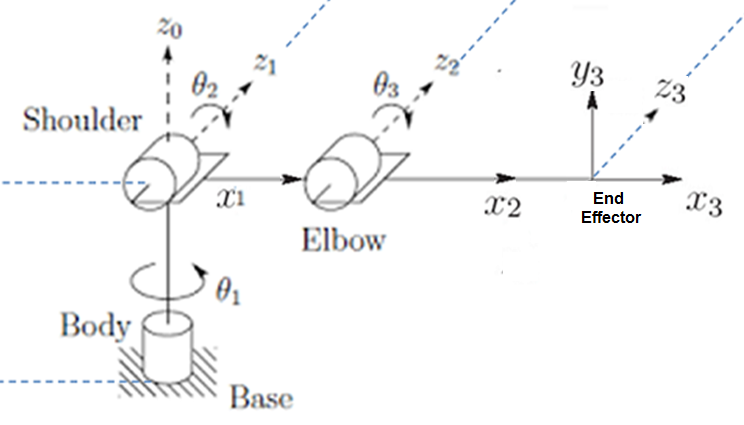
\includegraphics[scale=0.5]{3dof_robot}
            \end{center}

            \noindent This type of modeling allows for a simple and power description of the fundamental degrees of freedom and allowable motion which any robot arm of any construction can possess. This abstraction is vital for deriving the equations of motion (EOM) for an arbitrary robot arm, and lays the foundation for a useful parameterization (Denavit-Hartenberg Convention).\\

            \noindent By adopting this structure, the problem of deriving the dynamics and kinematics of the system reduces to a rather simple (if tedious) application of \underline{Lagrange Equation} for the full robot arm. Once these dynamics are obtained they can be used to compute the joint velocities, accelerations, and positions, given actuator inputs in the form of commanded torques, at each joint.

        \end{enumerate}


    \section*{Modeling}

    As previously mentioned, there exist reasonable methods to obtain the equations of motion for a robotic manipulator. This is important due to the project requirement that project is simulatable. Beyond this requirement however, the developement of the nolinear robot model is pivotal for the use of MPC, where the model itself is used to make predictions to determine the optimal controller inputs. \\


    \subsection*{Modeling Assumptions:}

    In order to keep the modeling of the robot simple this project plans to following the following simplications and assumptions.


        \begin{enumerate}
          \item \subsubsection*{Robot Construction Assumptions}

            Typically, simplified robot models are assumed to be construction of lower pairs including revolute or prismatic joints. Each member of the robots construction are assumed to be rigid bodies with no appreciable compliance. This formulation ensures that the robot is not an under actuated system, as well as keeping the dynamics simple and straightforward. These are reasonable assumptions for most robot manipulators of simple construction.

          \item \subsubsection*{Actuator Assumptions}

          With the exception of actuator saturation, this project will assume \underline{perfect} actuators, such that modeling of the actuators is not required and that if `X' Newton-meters of torque is commanded, the actuator will supply that amount granted that it does not exceed the saturation limits specified. This enables the controller to directly command the model by specifying joint torques.

        \item \subsubsection*{Sensor Assumptions}

        This project assumes perfect sensing of the system states. This is not an unreasonable assumption, since in most robots, servos and motors are encoded and require minimal effort to obtain relatively high accuracy positional information. Since it is assumed that the simulated actators haves have operating frequency above that of the controller, we can safely neglect sensor uncertainty in the simulations


        \end{enumerate}

\printbibliography

\end{document}
